% !TEX root =  manuscript.tex
\section{Methodology}\label{sec:methodology}

In order to conduct the survey in a thorough
and structured manner, we follow the established
guidelines by Kitchenham et al.~\cite{kitchenham2007guidelines}.
We begin by introducing terminology
and concepts needed to understand the remainder
of this survey.
Next, we define the scope of the work
and flesh it out into specific research questions
we aim to answer in this survey.
We then describe the details of the paper
collection process. 
Finally, we specify the inclusion and exclusion criteria
applied to select the most relevant body of work 
from the existing literature. 

\subsection{Definitions}\label{sec:defs}

In order to categorize
the use of visual approaches in software engineering, 
we use the terms \textit{areas} and \textit{tasks}.
Software engineering areas are the various stages in the software
lifecycle~\cite{IEEEComputerSociety:2014:GSE:2616205}.
Examples of SE areas include software requirements, software design,
and software testing.
Within each area, different \textit{tasks} can be defined.
Each task is a specific activity that aims to
achieve a well-defined objective related to that area.
For instance, we refer to unit testing or regression testing as
SE tasks within the software testing SE area,
whereas code migration or code refactoring are tasks within
software maintenance area.
Accordingly, the rationale for using these two terms is
to discuss our findings in more precise levels of granularity,
in order to be able to analyze the findings across areas and
for tasks within a specific area.

Next, we define the following terms in order to clarify
which aspect of computer vision is being discussed:

\begin{defn}[\textbf{Visual Artifact}]
\textit{A visual artifact is any datum %of information 
that satisfies the following two conditions: 
(1)~it constitutes a digital image or video, and
(2)~it is associated with one or more software engineering area(s).}
\end{defn}

\begin{defn}[\textbf{Visual Approach}]
\textit{A visual approach is an algorithm designed to solve a software engineering problem,
which takes as input one or more visual artifacts, 
then typically incorporates a computer vision method or similar techniques as one or more of its steps,
and finally yields an output that is used to achieve a software engineering task.
}
\end{defn}

The rationale for defining these two terms is to have
precision and clarity when describing how visual analysis is used to 
solve a software engineering problem.
We use the term \emph{visual approach} to indicate 
that the approach used to solve an SE problem 
is based on analyzing visual data pertaining to the software.
We use the term \emph{visual artifact} to refer to software artifacts
that are visual in nature, to differentiate them from other
software artifacts that are non-visual (e.g., log files,
requirements documents). 
The link between the two terms is that 
visual artifacts are the visual data consumed
by a visual approach.
Similarly, a visual approach is the algorithm
that needs visual artifacts as input. 
To clarify all of the aforementioned terms,
we give a simple example.  
Consider the case of cross-browser testing,
where the goal is to check whether a given
web app is being rendered identically in different browsers.
Visual approaches for cross-browser testing
often take a screenshot of the app in a set of 
different browsers, and then visually compare the screenshots.
In this case,
screenshots are the visual artifacts used or extracted
from the software,
and screenshot image comparison is the visual approach used to 
solve the SE task of cross-browser testing.

\subsection{Scope}\label{sec:scope}

The scope of this work is to conduct a survey
to help structure, curate, and unify
the dispersed literature in this research area,
and to analyze how computer vision techniques have
been used in software engineering,
and what challenges were reported when they were used. 
This would help shed light on the potential of these 
techniques, and make them more visible and accessible.

\changed{
\autoref{fig:scope} illustrates the scope of this work
in relation to the software engineering life cycle
and other software artifacts. 
The figure should be viewed as a multi-step process, 
beginning with visual artifacts construction, and ending with 
an application to a software engineering task, 
as defined in Section~\ref{sec:defs}.  
As shown in the figure,
the scope is to survey the following aspects: 
(1)~how are visual artifacts (defined in Section~\ref{sec:defs})
constructed or acquired from the software?  
%
This aspect is included in the scope because constructing or acquiring 
visual artifacts is the first step in a computer vision 
processing pipeline, and therefore should be explored 
in order to have a well-rounded survey.
%
(2)~what computer vision algorithms are used to analyze or 
process the constructed visual artifacts? 
% 
This aspect is included in the scope because examining the visual 
processing or analysis conducted in order to address a given paper's 
research questions yields insight into how visual techniques 
can be potentially applied to various tasks of software engineering.
%
(3)~what are the software engineering areas and tasks
where visual approaches have been used?

The figure also helps clarify what areas are outside the scope
of this survey.
For instance, the scope is not concerned with works where 
computer vision techniques were not utilized, 
or works that do not use any visual artifacts. 
Section \ref{sec:inclusions} fleshes out the scope into a detailed set of 
inclusion and exclusion criteria. 
}


\subsection{Research Questions}
As discussed in Section \ref{sec:scope},
the scope is to survey the use of computer vision
in solving software engineering problems.
In this section, we flesh out the scope
into the following specific research questions:

RQ1: What are the main software engineering areas and tasks
for which computer vision approaches have been used to date? 
We formulate this RQ in order to build a high level
picture of the areas of software engineering where computer vision
approaches were used. This aims at identifying potential trends
of areas with high adoption of computer vision 
and conversely areas where little to no computer vision approaches were used.
This can help the software engineering community in identifying
potential gaps in the utilization of computer vision for software engineering. 

RQ2: Why are computer vision approaches adopted? 
We formulate this RQ in order to identify common rationales 
for using computer vision to solve software engineering problems.
This understanding of why computer vision approaches
were used can subsequently help identify new software engineering
areas or tasks where similar problems and rationales exist
and therefore potentially benefiting from computer vision approaches.

RQ3: How are computer vision approaches applied to software and its visual artifacts? 
This RQ is a natural progression of the previous RQs. 
The previous RQs identified the rationales of using computer vision 
and the SE areas where computer vision were used.
This RQ examines the ``how.''
That is, the mechanism(s) by which computer vision was applied to software.
This can help guide the implementation of computer vision approaches
to solve software engineering problems.

RQ4: How are software engineering tasks that leverage computer vision techniques evaluated? 
This RQ examines the methods used to evaluate the use of computer vision approaches
in software engineering problems, as well as a summary of the reported limitations and challenges.
This may help with selecting an evaluation strategy when exploring the use of a computer vision approach,
and informing adopters of potential challenges.

\begin{figure*}
    \centering
    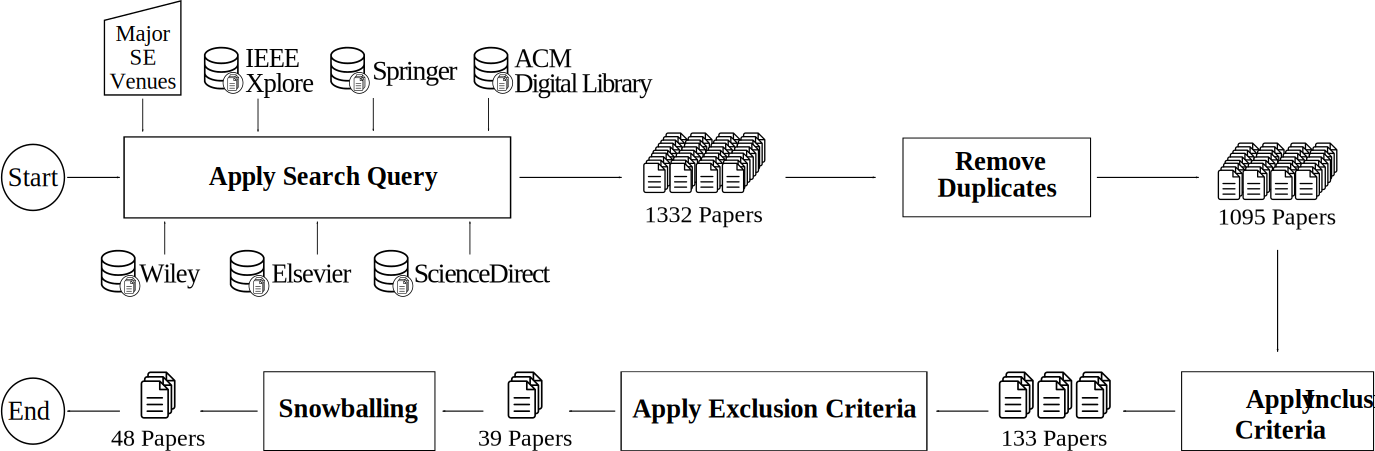
\includegraphics[width=0.80\textwidth]{survey/figures/overview}
    \caption{Overview of the paper collection process. }
    \label{fig:overview}
\end{figure*}

\subsection{Paper Collection}\label{sec:collection}

\autoref{fig:overview} shows our paper search and selection process.
In order to collect as much relevant literature as possible, 
we used two types of sources for paper collection: 
paper repository databases, and major software engineering venues.

\header{Paper Repository Databases}
To conduct our search, we used the databases of the following
well-known publishers of scientific literature:
IEEE Xplore, ACM Digital Library, ScienceDirect, Springer, Wiley, and Elsevier.
The search covers papers that have been published until June 2020. 
We used more than one database to ensure collecting
as many papers as possible from all known publishers.

\header{Software Engineering Venues}
The preceding selection of paper repositories
aims at casting a wide net in order to capture as many
relevant literature as possible.
However, since the databases contain an extremely large
number of papers, it is possible that papers 
relevant to our survey are lost in the vast number of returned papers.

For this reason, and in order to make sure we collect highly relevant papers, we complemented the database search with a manual issue-by-issue search within the conference proceedings and journal articles from 
top-tier software engineering venues (listed in \autoref{tbl:paper-sources}).
The final pool of collected papers is the combined list of papers from both the database search and the SE venues search.

\changed{
\header{Interdisciplinary Venues}
Given the interdisciplinary nature of this work, 
we also performed manual issue-by-issue search within 
the conference proceedings of relevant fields, namely, 
computer-human interaction, computer vision and machine 
learning. We selected the top three venues (based on the h5 index from Google Scholar) from each field.
The searched venues are listed in the last section of
 \autoref{tbl:paper-sources} (under ``Interdisciplinary Venues'').
}

\header{Search Query} For each of the aforementioned sources, 
we performed a search query using various combinations
of terms to retrieve papers in different software engineering areas
that are potentially using computer vision.
The query was performed on all data fields of the paper,
returning matches to either the \emph{title}, \emph{abstract},
\emph{keywords}, or \emph{text} of the paper.
The query is composed of two parts: keywords related to the approach
and keywords of the various software engineering areas.
Keywords of the approach include strings such as
``computer vision'' or ``visual''.
They were included in the query in order to indicate
our interest in works that use computer vision or visual approach.
Keywords describing the areas include strings such as
``development'' or ``testing'' or any of the software engineering
life cycle phases (e.g., requirements, maintenance).
The final applied search query is as follows:
%\begin{quote}
\emph{{[}computer vision {OR} image processing 
{OR} image analysis {OR} visual{]}
\ \ {AND}\ \ 
{[}requirements {OR} design {OR} development 
{OR} testing {OR} maintenance {OR} comprehension {]}}
%\end{quote}
The result of this query led to an initial pool of \initialPoolSize papers,
which was further filtered in the next stages.

\header{Duplicates removal}
During the paper collection step, we aimed to be
thorough by including as many paper sources as possible
in order to capture all potentially relevant works.
However, this resulted in many duplicate papers since a given
paper might be included in more than one database and venue.
Therefore, we filtered the collected pool
of papers by removing duplicate works based on their titles.

\subsubsection{Inclusion and Exclusion Criteria}\label{sec:inclusions} 
The search conducted on the databases and venues is, 
by design, very inclusive. This allows us to collect as many
papers as possible in our pool. 
However, this generous inclusivity results in having papers that are not directly
related to the scope of this survey.
Accordingly, we define a set of specific inclusion and exclusion criteria
and apply them to each paper in the pool, and remove papers not meeting the criteria.
This ensures that each collected paper is inline with our scope and research questions.

\header{Inclusion criteria}
We define the following inclusion criteria: 
%
(1)~The paper should be contributing to any stage
of the software engineering process,
whether in early requirements and modeling,
through development and design, or finally testing and maintenance.
We included this criteria in order to focus on software engineering papers.
This is because we found a notable number of computer vision papers 
that were in fields other than software engineering (e.g., biology).
%
(2)~The paper should include a computer vision processing of the software or its artifacts.
That is, the work achieves its objective (whether partially or fully) by extracting,
analyzing, or processing visual artifacts pertaining or relevant to the software.
This is an important and key criterion for paper selection because it ensures
we meet the core scope of our survey. 
%
(3)~The paper should be a full technical research paper that has a
detailed description of the visual approach utilized.
This criterion is imposed in order to have sufficient information to answer our research questions.
Answering our research questions, such as RQ3 and RQ4, requires that 
we examine technical software engineering research papers,
as opposed to, for instance,
technical magazine articles, industrial white papers, or similar grey literature
which do not have sufficient level of detail.
Some demo/short papers can be allowed if they have dedicated and detailed 
sections discussing the detailed mechanism of the visual approach and its
evaluation. 
This enables creating a pool of papers that have
rich and detailed information and findings,
in order to answer key research questions related to
the details of the visual approach, the process of creating visual artifacts,
and evaluation strategies. 
%
(4)~The paper should contain a section dedicated to illustrating
some form of quantitative or qualitative evaluation of the technique,
or an illustration of its use case. 
This criterion was imposed in order to enable us to
fully answer and explore our research questions regarding evaluation strategies.

These criteria were applied 
in a group review process by the authors.
For each paper in the pool, each author initially checked the title and abstract,
and briefly examined the proposed approach and results to ensure that it meets the inclusion criteria.
If this check was not sufficient to conclusively decide
whether the paper should be included in the pool,
we proceeded with a secondary in-depth examination of
the paper's objective, methodology, and evaluation to ensure that the inclusion criteria were met.
Finally, a discussion among the authors was triggered,
to decide on the inclusion of the paper in the final list of works.
 
% !TEX root =  manuscript.tex

\begin{table}

\revised{0.99\textwidth}{

\caption{Conference proceedings and journals considered for paper collection (in addition to database search).}
\centering
% \small % bigger
\scriptsize %smaller
% \tiny % much smaller
\renewcommand{\arraystretch}{1.2}
\setlength{\tabcolsep}{2.5pt}

\begin{tabular}{l l p{7.5cm}}
	\toprule
	& \textbf{Acronym}   & \textbf{Venue}                                                                                              \\ \midrule
	\multirow{18}{*}{\rotatebox{90}{\textbf{SE Conferences}}}
	& ICSE          & International Conference on Software Engineering                                                            \\
	& FSE           & International Symposium on Foundations of Software Engineering                                  \\
	& ESEC/FSE	    & Joint European Software Engineering Conference and Symposium on the Foundations of Software Engineering \\
	& ASE           & International Conference on Automated Software Engineering                                         \\
	& ESEM          & International Symposium on Empirical Software Engineering and Measurement                         \\
	& ICST          & International Conference on Software Testing, Verification and Validation                              \\
	& ISSTA         & International Symposium on Software Testing and Analysis                                        \\
	& MSR           & International Conference on Mining Software Repositories                                                    \\
	& RE            & International Requirements Engineering Conference                                                      \\
	& ICSME         & International Conference on Software Maintenance and Evolution                                          \\
	& MODELS        & International Conference on Model Driven Engineering Languages and Systems                         \\
	& ISSRE         & International Symposium on Software Reliability Engineering                                            \\
	& EASE          & Evaluation and Assessment in Software Engineering                                                           \\
	% & UIST          & ACM Symposium on User Interface Software and Technology                                                     \\
	% & WWW           & International World Wide Web conference                                                                     \\
	% & WSDM          & ACM International Conference on Web Search and Data Mining                                                  \\
	% & ICWE          & International Conference on Web Engineering                                                                 \\
	% & CHI           & ACM CHI Conference on Human Factors in Computing Systems                                                    \\ \midrule
	\midrule
	\multirow{12}{*}{\rotatebox{90}{\textbf{SE Journals}}}
	& TSE           & Transactions on Software Engineering                                                                   \\
	& EMSE          & Empirical Software Engineering                                                                              \\
	& TOSEM         & Transactions on Software Engineering and Methodology                                                    \\
	& JSS           & Journal of Systems and Software                                                                             \\
	% & JVLC          & Journal of Visual Languages and Computing                                                                   \\
	& JSEP          & Journal of Software: Evolution and Process                                                                  \\
	& STVR          & Software Testing, Verification and Reliability                                                              \\
	& ASE           & Automated Software Engineering                                                                              \\
	& IEEE SOFTWARE & IEEE Software                                                                                               \\
	& IET SOFTW.    & IET Software                                                                                                \\
	& IST           & Information and Software Technology                                                                         \\
	& SQJ           & Software Quality Journal                                                                                    \\ 


	\midrule
	
	\multirow{10}{*}{\rotatebox{90}{\textbf{Interdisciplinary Venues}}}
	& CHI       & Conference on Human Factors in Computing Systems  	\\
	& CSCW 		& Conference on Computer-Supported Cooperative Work 	\\
	& UbiComp	& Conference on Pervasive and Ubiquitous Computing 		\\ 
	& UIST      & Symposium on User Interface Software and Technology  	\\

	& NeurIPS   & Conference on Neural Information Processing Systems   \\
	& ICLR		& International Conference on Learning Representations  \\
	& ICML		& International Conference on Machine Learning			\\

	& CVPR    & Conference on Computer Vision and Pattern Recognition   \\
	& ECCV	  & European Conference on Computer Vision					\\
	& ICCV		& International Conference on Computer Vision		\\
	
	\bottomrule

	\end{tabular}
	\label{tbl:paper-sources}
}
\end{table}


\header{Exclusion criteria}\label{sec:exclusions}
During our initial experimental test rounds of paper searching,
we observed that a relatively large number of retrieved papers
were on visualization research.
This is understandable and expected because our queries
include terms such as image, visual, and design.

Accordingly, we exclude papers published in the area of software
visualization for the following reasons.
First, the visualization class of algorithms does not
constitute a \emph{visual approach}, as defined in Section~\ref{sec:defs}.
Visualizations do not use any visual artifact of the software \emph{as an input}.
Rather, such work performs a final visual output or visual
representation of a complete, non-visual, approach.
Accordingly, this area of research is excluded
since it would be outside the scope of this work.
We recall that the scope is to survey visual approaches which,
by definition, \emph{consume} visual artifacts pertaining to the software during the
course of running their algorithm or processing.
Second, in addition to visualization being outside the scope of this survey,
it is already a well-known and common aspect of software engineering, 
and plenty of surveys already exist on the use of visualization
in various aspects of software engineering, 
as mentioned in \Cref{sec:related}.

We also exclude commercial software services or open-source tools
that have no corresponding publication, for the following reasons.
First, including services or tools that are not peer-reviewed
would negatively impact our ability to conduct the survey because tools and services 
that are not backed by a publication do not include
a detailed explanation of their approach.
This reduces our ability to answer key research questions for this survey,
such as what specific computer vision techniques were used,
what is the visual artifacts construction process, and 
how were the computer vision algorithms applied to the visual artifacts.
Services and tools without a corresponding publication
also typically do not have a thorough systematic evaluation,
and therefore we are unable to answer research questions related to
how computer vision techniques were evaluated,
what are the main findings, and what were the challenges.


\header{Snowballing}
At the end of searching database repositories and
conference proceedings and journals,
and applying inclusion and exclusion criteria,
we obtained a total of 57 unique papers.
Next, 
to mitigate the risk of omitting relevant literature from this survey,
we also performed backward snowballing~\cite{Wohlin:2014:GSS:2601248.2601268}
by inspecting the references cited by the collected papers so far.
Nine additional papers were retrieved during this phase,
which led to a final pool of 66 unique papers.
\autoref{table:selected-primary-studies}
shows the final pool of papers
that will be discussed and analyzed in the remainder of this work.

% !TEX root =  manuscript.tex

\begin{table}[t]
\caption{Collected data items (Synthesis Matrix)}
\centering
\renewcommand{\arraystretch}{1.2}
\setlength{\tabcolsep}{9pt}
\begin{tabular}{l l}
	\toprule
	\textbf{Field}                    & \textbf{Use}     \\ \midrule
	Title                             & Documentation    \\
	Author(s)                         & Documentation    \\
	DOI identification number         & Documentation   \\
	Abstract                          & Paper Selection \\
	Text                          & Paper Selection \\
	Venue                             & RQ1             \\
	Year                              & RQ1             \\
	% Total number of Citations         & \davood{?}      \\
	Target platform                   & RQ1             \\
	Software engineering area         & RQ1             \\
	Software engineering task         & RQ1             \\
	Reasons for adopting CV approach  & RQ2             \\
	Visual artifact(s) used           & RQ3             \\
	CV algorithm(s) used    	      & RQ3             \\
	Evaluation process \& challenges  & RQ4             \\
	Main results                      & RQ4             \\
	Limitations of CV methods used    & RQ4             \\ \bottomrule
\end{tabular}
	\label{tbl:collected-info}
\end{table}


\header{Extracted Information}
For each retrieved paper,
we collect a set of data necessary to answer the research questions. 
\autoref{tbl:collected-info} shows the list of data
collected from each paper
and their mapping to each research question.
As shown in the table,
the title, author(s), and document ID were used
for documentation purposes to keep track of the various papers.
The abstract and text were used for the paper selection process
and applying the inclusion and exclusion criteria.
The venue, year, software engineering area and task
of each paper was also collected in order to discuss and answer
RQ1. 
We also extract the target platform for each paper, which is  
the type of computing device (e.g., desktop, mobile) that the 
analyzed software runs on.
A list of reasons for adopting computer vision was also 
extracted from each paper in order to answer RQ2.
The visual artifact(s) and the visual approach utilized
were also identified in each paper in order to discuss RQ3.
Finally, we log the evaluation process and the results and findings
from each collected paper in order to answer RQ4.
All these data are collected, analyzed, and used to synthesize 
the findings for the rest of this survey. 
In order to facilitate the use of this data by
the general research community, the data have been 
made publicly available at http://tiny.cc/tse-2020.

% !TEX root =  manuscript.tex
\begin{sidewaystable}
%\begin{table*}
%\scriptsize
\tiny
\renewcommand{\arraystretch}{1.0}
\setlength{\tabcolsep}{4.5pt}
%\revised{1.01\textwidth}{
\caption{Collected pool of papers (in chronological order).}
\label{table:selected-primary-studies}
\begin{tabular}{@{} lp{12.9cm}ll @{}}
%\begin{longtable}{@{} lp{12.9cm}ll @{}}
\toprule
\textbf{Reference}           & \textbf{Title}                                                                                                                      & \textbf{Venue} & \textbf{Year} \\  

\midrule

% \rowcolor{\hlcolor}
\citet{Landay-2001-IEEEComputer}       & Sketching Interfaces: Toward More Human Interface Design                                                                  & IEEE Computer  & 2001          \\
\citet{Caetano-2002-AAAI}    & JavaSketchIt: Issues in Sketching The Look of User Interfaces                                                                       & AAAI           & 2002          \\
% \rowcolor{\hlcolor}
\citet{Fails-2003-CHI}       & A Design Tool for Camera-based Interaction                                                                                          & CHI            & 2003          \\

\citet{Coyette-2007-INTERACT}& Multi-fidelity Prototyping of User Interfaces                                                                                       & INTERACT       & 2007          \\

% \rowcolor{\hlcolor}
\citet{Zheng-2009-CHI}       & Correlating Low-level Image Statistics with Users - Rapid Aesthetic and Affective Judgments of Web Pages                            & CHI            & 2009          \\
\citet{Chang-2010-CHI}       & GUI Testing Using Computer Vision                                                                                                   & CHI            & 2010          \\
\citet{Choudhary-2010-ICSM}  & WEBDIFF: Automated Identification of Cross-browser Issues in Web Applications                                                       & ICSM           & 2010          \\
\citet{Li-2010-CHI}          & FrameWire: A Tool for Automatically Extracting Interaction Logic from Paper Prototyping Tests                                       & CHI            & 2010          \\
% \rowcolor{\hlcolor}
\citet{Dixon-2010-CHI}       & Prefab: Implementing Advanced Behaviors using Pixel-based Reverse Engineering of Interface Structure                                & CHI            & 2010          \\

\citet{Delamaro-2011-STVR}   & Using Concepts of Content‐based Image Retrieval to Implement Graphical Testing Oracles                                              & STVR           & 2011          \\
\citet{Dixon-2011-CHI}       & Content and Hierarchy in Pixel-based Methods for Reverse Engineering Interface Structure                                            & CHI            & 2011          \\
\citet{Seifert-2011-MobileHCI} & Mobidev: A Tool for Creating Apps on Mobile Phones                                                                                & MobileHCI      & 2011          \\
\citet{Choudhary-2012-ICST}  & Crosscheck: Combining Crawling and Differencing to Better Detect Cross-browser Incompatibilities in Web Applications                & ICST           & 2012          \\

% \rowcolor{\hlcolor}
\citet{Givens-2013-ICSE}     & Exploring The Internal State of User Interfaces by Combining Computer Vision Techniques with Grammatical Inference                  & ICSE           & 2013          \\

% \rowcolor{\hlcolor}
\citet{Liang-2013-UIST}      & SeeSS: Seeing What I Broke -- Visualizing Change Impact of Cascading Style Sheets (CSS)                                             & UIST           & 2013          \\


\citet{Scharf-2013-ICSE}     & Dynamic Injection of Sketching Features Into GEF-based Diagram Editors                                                              & ICSE           & 2013          \\
\citet{Alegroth-2013-ICST}   & JAutomate: A Tool for System- and Acceptance-test Automation                                                                        & ICST           & 2013          \\
\citet{Semenenko-2013-ICSM}  & Browserbite: Accurate Cross-Browser Testing via Machine Learning over Image Features                                                & ICSM           & 2013          \\
\citet{Choudhary-2013-ICSE}  & X-PERT: Accurate Identification of Cross-Browser Issues in Web Applications                                                         & ICSE           & 2013          \\
\citet{Lin-2014-TSE}         & On the Accuracy, Efficiency, and Reusability of Automated Test Oracles for Android Devices                                          & TSE            & 2014          \\
\citet{Mahajan-2014-ASE}     & Finding HTML Presentation Failures Using Image Comparison Techniques                                                                & ASE            & 2014          \\
\citet{Amalfitano-2014-WISE} & Towards Automatic Model-in-the-loop Testing of Electronic Vehicle Information Centers                                               & WISE           & 2014          \\
\citet{Selay-2014-DICTA}     & Adaptive Random Testing for Image Comparison in Regression Web Testing                                                              & DICTA          & 2014          \\

% \rowcolor{\hlcolor}
\citet{Bao-2015-ICSE}        & scvRipper: Video Scraping Tool for Modeling Developers' Behavior Using Interaction Data                                             & ICSE           & 2015          \\

\citet{Nguyen-2015-ASE}      & Reverse Engineering Mobile Application User Interfaces with REMAUI                                                                  & ASE            & 2015          \\
\citet{Burg-2015-UIST}       & Explaining Visual Changes in Web Interfaces                                                                                         & UIST           & 2015          \\
\citet{Mahajan-2015-ICST}    & Detection and Localization of HTML Presentation Failures Using Computer Vision-Based Techniques                                     & ICST           & 2015          \\
\citet{Hori-2015-SEKE}       & An Oracle based on Image Comparison for Regression Testing of Web Applications                                                      & SEKE           & 2015          \\

% \rowcolor{\hlcolor}
\citet{Reinecke-2016-CHI}    & Enabling Designers to Foresee Which Colors Users Cannot See                                                                         & CHI            & 2016          \\

\citet{Deka-2016-UIST}       & ERICA: Interaction Mining Mobile Apps                                                                                               & UIST           & 2016          \\
\citet{Ponzanelli-2016-ICSE} & Too Long; Didn’t Watch! Extracting Relevant Fragments from Software Development Video Tutorials                                     & ICSE           & 2016          \\
\citet{Mahajan-2016-ICST}    & Using Visual Symptoms for Debugging Presentation Failures in Web Applications                                                       & ICST           & 2016          \\
\citet{Feng-2016-ASE}        & Multi-objective Test Report Prioritization Using Image Understanding                                                                & ASE            & 2016          \\
\citet{Patric-2016-ASE}      & Automatic Test Image Generation Using Procedural Noise                                                                              & ASE            & 2016          \\
\citet{He-2016-ICWS}         & X-Check: A Novel Cross-browser Testing Service Based on Record/Replay                                                               & ICWS           & 2016          \\

\citet{Deka-2017-UIST}       & Rico: A Mobile App Dataset for Building Data-Driven Design Applications                                                             & UIST           & 2017          \\
\citet{Wan-2017-STVR}        & Detecting Display Energy Hotspots in Android Apps                                                                                   & STVR           & 2017          \\
\citet{Bao-2017-EMSE}        & Extracting and Analyzing Time-series HCI Data from Screen-captured Task Videos                                                      & EMSE           & 2017          \\
\citet{Zhang-2017-ASE}       & Sketch-guided GUI Test Generation for Mobile Applications                                                                           & ASE            & 2017          \\
\citet{Chen-2017-IUI}        & UI X-Ray: Interactive Mobile UI Testing Based on Computer Vision                                                                    & IUI            & 2017          \\

% \rowcolor{\hlcolor}
\citet{Wu-2017-CSCW}         & Automatic Alt-text: Computer-generated Image Descriptions for Blind Users on a Social Network Service                               & CSCW           & 2017          \\


\citet{Reiss-2018-ASEj}      & Seeking the User Interface                                                                                                          & ASE J.         & 2018          \\
\citet{Kirac-2018-JSS}       & VISOR: A Fast Image Processing Pipeline with Scaling and Translation Invariance for Test Oracle Automation of Visual Output Systems & JSS            & 2018          \\
\citet{Leotta-2018-STVR}     & Pesto: Automated Migration of DOM‐based Web Tests Towards the Visual Approach                                                       & STVR           & 2018          \\
\citet{canvas_icst2018}   & Web Canvas Testing through Visual Inference                                                                                         & ICST           & 2018          \\
\citet{Xu-2018-TOIT}         & Cross-Browser Differences Detection Based on an Empirical Metric for Web Page Visual Similarity                                     & TOIT           & 2018          \\
\citet{Kuchta-2018-EMSE}     & On the Correctness of Electronic Documents: Studying, Finding, and Localizing Inconsistency Bugs in PDF Readers and Files           & EMSE           & 2018          \\
\citet{Bao-2018-TSE}         & VT-Revolution: Interactive Programming Video Tutorial Authoring and Watching System                                                 & TSE            & 2018          \\
\citet{Moran-ICSE-2018}      & Automated Reporting of GUI Design Violations for Mobile Apps                                                                        & ICSE           & 2018          \\

% \rowcolor{\hlcolor}
\citet{Chen-2018-ICSE}       & From UI Design Image to GUI Skeleton: A Neural Machine Translator to Bootstrap Mobile GUI Implementation                            & ICSE           & 2018          \\

% \rowcolor{\hlcolor}
\citet{Sun-2018-ICML}        & Neural Program Synthesis from Diverse Demonstration Videos                                                                          & ICML           & 2018          \\

% \rowcolor{\hlcolor}
\citet{Lim-2018-UIST}        & Ply: A Visual Web Inspector for Learning from Professional Webpages                                                                 & UIST           & 2018          \\

\citet{Moran-TSE-2018}       & Machine Learning-Based Prototyping of Graphical User Interfaces for Mobile Apps                                                     & TSE            & 2018          \\
\citet{Stocco-2018-FSE}      & Visual Web Test Repair                                                                                                              & FSE            & 2018          \\
\citet{Tanno-2018-ICSTW}     & Support for Finding Presentation Failures by Using Computer Vision Techniques                                                       & ICST           & 2018          \\
\citet{bajammal2018generating}    & Generating Reusable Web Components from Mockups                                                                                     & ASE            & 2018          \\
\citet{Moran-2018-ASE}       & Detecting and Summarizing GUI Changes in Evolving Mobile Apps                                                                       & ASE            & 2018          \\
\citet{Natarajan-2018-MOBILESoft} & P2A: A Tool for Converting Pixels to Animated Mobile Application User Interfaces                                               & MOBILESoft     & 2018          \\
\citet{Osman-2018-SEAA}      & An Automated Approach for Classifying Reverse-engineered and Forward-engineered UML Class Diagrams                                  & SEAA           & 2018          \\
\citet{Xiao-2019-ICSE}       & Automatic Identification of Sensitive UI Widgets based on Icon Classification for Android Apps                                      & ICSE           & 2019          \\ 
\citet{Huang-2019-CHI}       & Swire: Sketch-based User Interface Retrieval                                                                                        & CHI            & 2019          \\

% \rowcolor{\hlcolor}
\citet{Zhao-2019-ICSE}       & ActionNet: Vision-Based Workflow Action Recognition from Programming Screencasts                                                    & ICSE           & 2019          \\

% \rowcolor{\hlcolor}
\citet{Yu-2019-ASE}          & LIRAT: Layout and Image Recognition Driving Automated Mobile Testing of Cross-Platform                                              & ASE            & 2019          \\

% \rowcolor{\hlcolor}
\citet{Swearngin-2019-CHI}   & Modeling Mobile Interface Tappability using Crowdsourcing and Deep Learning                                                         & CHI            & 2019          \\

% \rowcolor{\hlcolor}
\citet{Yuan-2020-CHI}        & Modeling Human Visual Search Performance on Realistic Webpages using Analytical and Deep Learning Methods                           & CHI            & 2020          \\

% \rowcolor{\hlcolor}
\citet{Wu-2020-CHI}          & Predicting and Diagnosing User Engagement with Mobile UI Animation via a Data-Driven Approach                                       & CHI            & 2020          \\ 

\bottomrule 

%\end{longtable}
\end{tabular}
%}
%\end{table*}
\end{sidewaystable}
